\documentclass[a4paper]{article}

\usepackage[english]{babel}
\usepackage[utf8]{inputenc}
\usepackage{fullpage}
\usepackage{amsmath}
\usepackage{graphicx}
\usepackage[colorinlistoftodos]{todonotes}
%\usepackage{hyperref}
\usepackage{amssymb}
\usepackage{subfigure}
\usepackage{url}
\usepackage[pagebackref=true,colorlinks,linkcolor=red,citecolor=green,breaklinks=true,bookmarks=false]{hyperref}
\usepackage{outline} 
\usepackage{pmgraph} \usepackage[normalem]{ulem}
\usepackage{graphicx} \usepackage{verbatim}
\usepackage{indentfirst}
\setlength{\parindent}{2em}
% \usepackage{minted} % need `-shell-escape' argument for local compile

\title{
    \vspace*{1in}
    
\includegraphics[width=2.75in]{figures/zhenglab-logo} \\
    \vspace*{1.2in}
    \textbf{\huge Weekly Work Report}
    \vspace{0.2in}
}

\author{Hongzhi Liu \\
    \vspace*{0.5in} \\
    \textbf{VISION@OUC} \\
    \vspace*{1in}
}

\date{\today}


\begin{document}
\par
\maketitle
\setcounter{page}{0}
\thispagestyle{empty}
\newpage


\section{Research problem}

During this period of week, I spend time studying deep learning and working about Faster R-CNN algorithm with CPU for URPC2018.

\section{Research approach}

For deep learning, I watch videos and write down the issues which I think are much important for further research. As for URPC2018, I need to learn about Faster R-CNN algorithm \cite{Ren2015Faster} and try to build environment on my laptop to run a demo.

\section{Research progress}

This week for deep learning course of Anandrew Ng, I know how to set up a neural network of a hidden layer and initialize the parameters. Besides, I learn to make predicitons using forward propagation as well as compute derivatives and apply gradient descent using back propagation. The details are in following sections. Furthermore, I have succeed in running a Faster R-CNN demo on my laptop with CPU which I take efforts to achieve this goal. 

\subsection{Binary Classification}

Logistic regression is an algorithm for binary classification. So we start by setting up the problem with an example of a binary classification problem. We have an input of an image and want to output a label to recognize this image as either being a cat, in which case we output 1 or not-cat in which case you output 0 and we're going to use y to denote the output label.

Computer stores three separate matrices to store an image corresponding to the red, green and blue color channels of this image. So if your input image is $64\times 64pixels$, then you would have 3 $\times$ 64 $\times$ 64 matrices corresponding to the red, green and blue pixel intensity values for your images. Although to make this little slide as much smaller matrices, which actually should be 64 $\times$ 64 matrices rather than 5 $\times$ 4 as shown in Fig.~\ref{p1}\subref{p1a}.
\begin{figure}[b] 
	\centering 
	\subfigure[]{ 
		\label{p1a} %% label for first subfigure 
		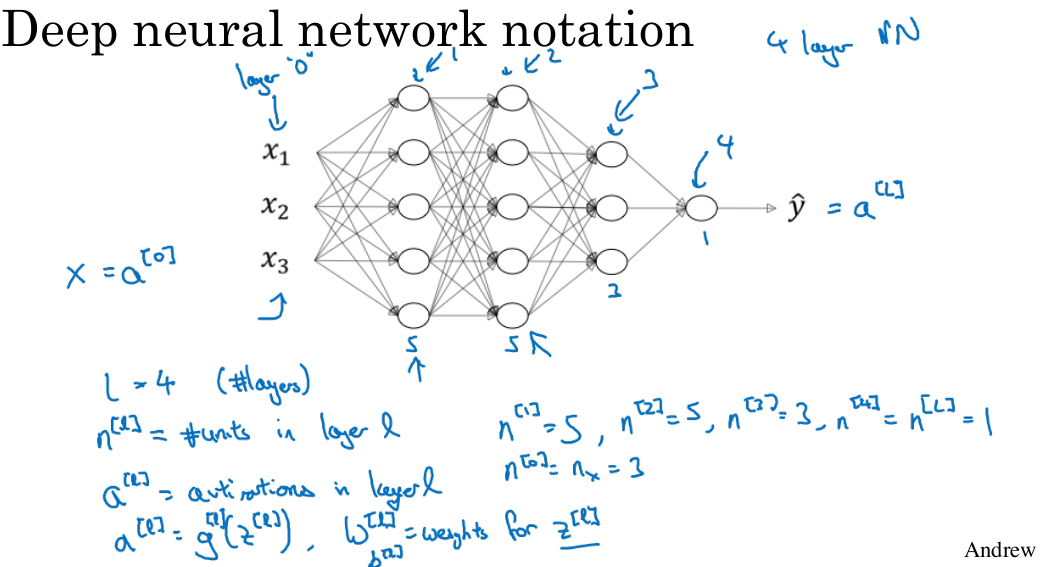
\includegraphics[scale=0.3]{figures/1.png} 
	} 
	\subfigure[]{ 
		\label{p1b} %% label for second subfigure 
		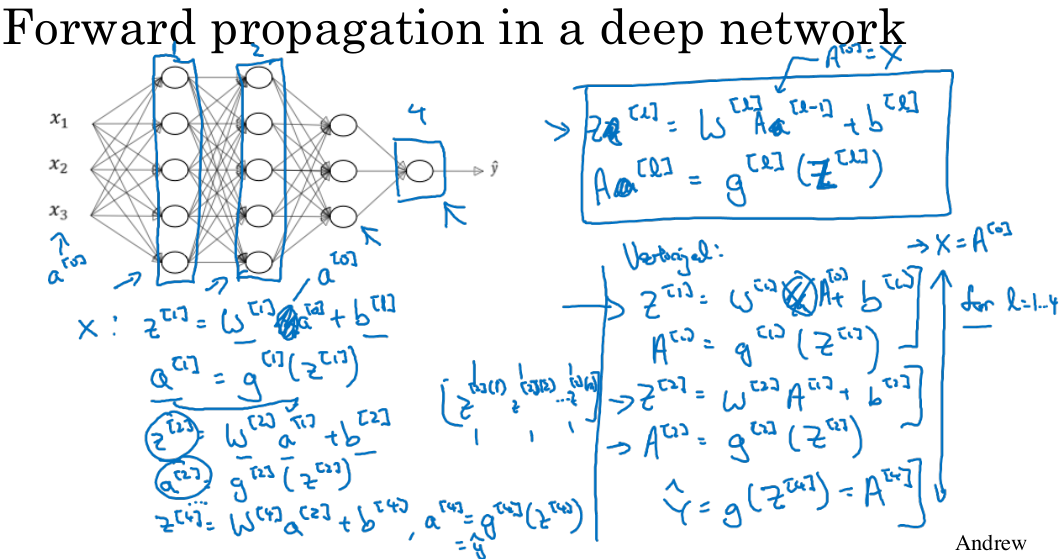
\includegraphics[scale=0.3]{figures/2.png} 
	} 
	\caption{An example of a binary classification problem} 
	\label{p1} %% label for entire figure 
\end{figure}
So to turn these pixel intensity values into a feature vector. We're just going to take all the pixel values 255, 231 and so on until we list all the red pixels. And then eventually 255, 134 and so on until we get a long feature vector listing out all the red, green and blue pixel intensity values of this image as shown in Fig.~\ref{p1}\subref{p1b}. If this image is a 64 $\times$ 64 image, the total dimension of this vector x will be 64 by 64 $\times$ 3 because that's the total numbers we have in all of these matrixes. Which in this case, turns out to be 12,288 that's what we get if multiply all those numbers as Fig.~\ref{p1}\subref{p1a}. 

And so we're going to use $n_x=12288$ to represent the dimension of the input features x. And sometimes for brevity, I will also just use n to represent the dimension of this input feature vector. So in binary classification, our goal is to learn a classifier that can input an image represented by this feature vector x. And predict whether the corresponding label y is 1 or 0, that is, whether this is a cat image or a non-cat image in this example.

A single training example is represented by a pair $(x,y)$ where x is an x-dimensional feature vector and the label y is either 0 or 1. Our training sets will comprise lower-case m training examples. So training sets will be written $(x(1), y(1))$ which is the input and output for the first training example and $(x(2), y(2))$ for the second training example up to $(x(m), y(m))$ which is your last training example as shown in Fig.~\ref{p2}. And then that altogether is our entire training set. Sometimes to emphasize that this is the number of train examples, we might write this as $M = M_{train}$. And when we talk about a test set, we might sometimes use $m$ subscript test to denote the number of test examples.
\begin{figure}
	\begin{center}
		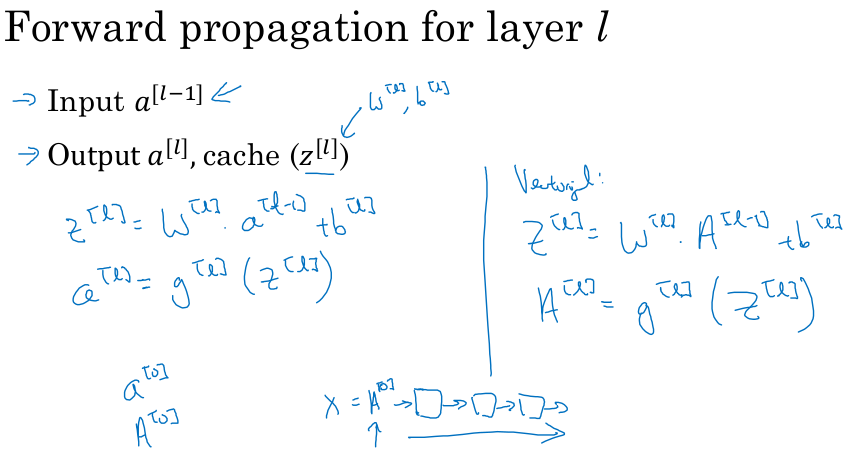
\includegraphics[scale=0.4]{figures/3.png}
	\end{center}
	\caption{Notation for a regression and for neural networks networks later in the course.}
	\label{p2}
\end{figure}
Finally, to output all of the training examples into a more compact notation, we're going to define a matrix, capital X. As defined by taking you training set inputs $x^1$, $x^2$ and so on and stacking them in columns. So we take $X^1$ and put that as a first column of this matrix, $X^2$, put that as a second column and so on down to $X^m$, then this is the matrix capital $X$.

When you implement this in Python, you see that x.shape, that's the python command for finding the shape of the matrix, that this an $(n_x, m)$. That just means it is an $n_x$ by $m$ dimensional matrix. So we're going to define capital Y to be equal to $Y_1$, $Y_2$, up to $Y_m$ like so. So Y here will be a 1 by m dimensional matrix as shown in Fig.~\ref{p2}.

\subsection{Logistic Regression and Cost Function}

This logistic regression is a learning algorithm that you use when the output labels Y in a supervised learning problem are all either zero or one, so for binary classification problems. If X is a picture, as we saw in the example, $\hat{y}$ tells us what is the chance that this is a cat picture. X an dimensional vector, given that the parameters of logistic regression will be W which is also an X dimensional vector, together with b which is just a real number as shown on the left in Fig.~\ref{p3}.
\begin{figure}
	\begin{center}
		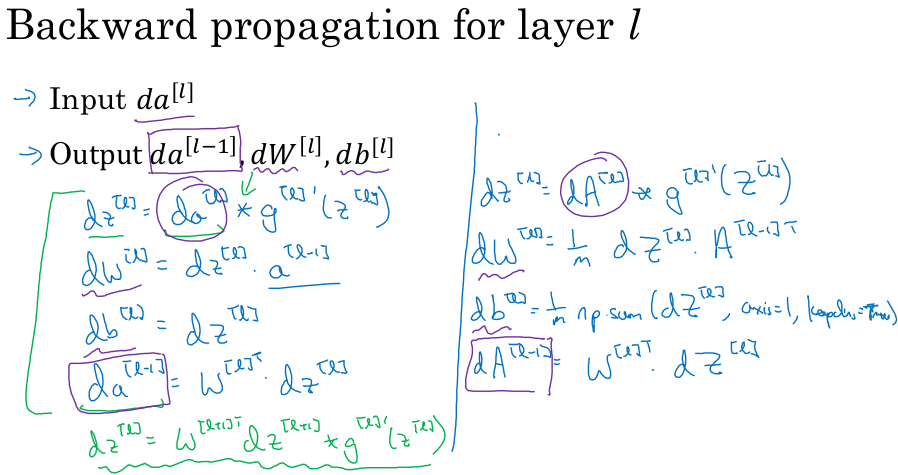
\includegraphics[scale=0.4]{figures/4.png}
	\end{center}
	\caption{The logistic regression.}
	\label{p3}
\end{figure}

In logistic regression, our output is instead going to be $\hat{y}$ equals the sigmoid function applied to this quantity. The sigmoid of Z looks like on the bottom left in Fig.~\ref{p3} and we're going to use Z to denote this quantity, $Z=W^\mathrm{T}x^{(i)}+b$ a formula for the sigmoid function as output above. If Z is very large, sigmoid of Z is close to 1. On the contrary,if Z is very small or a very large negative number,then sigmoid of Z is close to zero. So when we implement logistic regression, our job is to try to learn parameters W and b so that $\hat{y}$ becomes a good estimate of the chance of Y being equal to one.

When we programmed neural networks, we'll usually keep the parameter W and parameter b separate, where b corresponds to an interspectrum. As we saw the logistic regression model, in order to train the parameters W and b of the logistic regression model, you need to define a cost function. In logistic regression, we will actually define a different loss or error function that plays a similar role as squared error, that will give us an optimization problem that is convex and so we'll see in later which becomes much easier to optimize. What we use in logistic regression is actually the following loss or error function which is as Eq.~\ref{q1}.
\begin{equation}
\mathcal{L}(\hat{y}^{(i)},y^{(i)})=-[(y^{(i)}\log \hat{y}^{(i)})+(1-y^{(i)})\log(1-\hat{y}^{(i)})]   \label{q1}
\end{equation}

To understand why this makes sense, there are two cases to pay attention. In the first case, Y is equal to one then the loss function $L(\hat{y}^{(i)},y^{(i)})=-\log \hat{y}$. So this says if $y = 1$ you want $\log \hat{y}$ to be as large as possible and that means you want $\hat{y}$ to be close to one as well. The other case is if $y = 0$, then the loss function $L(\hat{y}^{(i)},y^{(i)})=-\log(1-\hat{y})$. And so if in learning procedure we try to make the loss function small, what this means is that you want $\log(1-\hat{y})$ to be large. We can conclude that this loss function is trying to make $\hat{y}$ as close to zero as possible which we can see in Fig.~\ref{p4}. In a word, The loss function was defined with respect to a single training example. It measures how well we're doing on it. 
\begin{figure}
	\begin{center}
		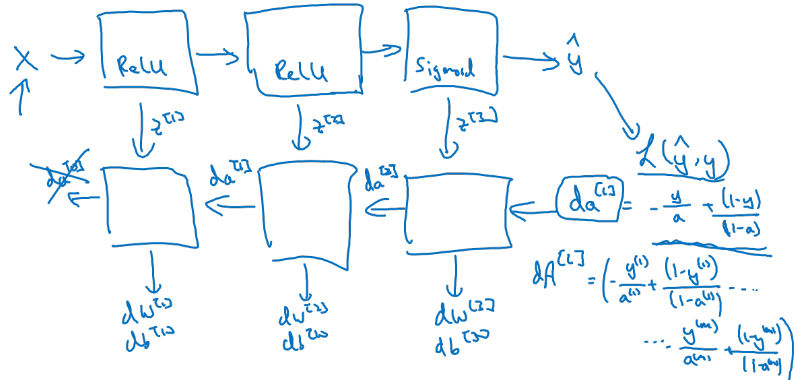
\includegraphics[scale=0.4]{figures/5.png}
	\end{center}
	\caption{Logistic regression cost function.}
	\label{p4}
\end{figure}

Besides, cost function which measures how well we're doing an entire training set. The cost function $J(w,b)=-\frac{1}{m}\sum_{i=1}^{m}[(y^{(i)}\log \hat{y}^{(i)})+(1-y^{(i)})\log(1-\hat{y}^{(i)})]$ is going to be the average with one of the m of the sum of the loss function applied to each of the training examples and turn as shown in Fig.~\ref{p4}. While here $\hat{y}$ is of course the prediction output by your logistic regression algorithm using a particular set of parameters W and b. So the terminology I'm going to use is that the loss function is applied to just a single training example like in Fig.~\ref{p4}. And the cost function is the cost of your parameters. 

Therefore, in training our logistic regression model, we're going to try to find parameters W and b that minimize the overall costs of machine J written at the bottom in Fig.~\ref{p4}.

\subsection{Gradient Descent}

Then I learn how to use the gradient descent algorithm to train or to learn the parameters w and b on your training set. We have on the second line the cost function J which is a function of parameters w and b then it is defined as the average. So in order to learn the set of parameters w and b, it seems natural that we want to find w and b that make the cost function $J(w,b)$ as small as possible. So here's an illustration of gradient descent as shown in Fig.~\ref{p5} and the height of the surface represents the value of $J(w,b)$ at a certain point. What we want to do is really to find the value of w and b that corresponds to the minimum of the cost function J.
\begin{figure}
	\begin{center}
		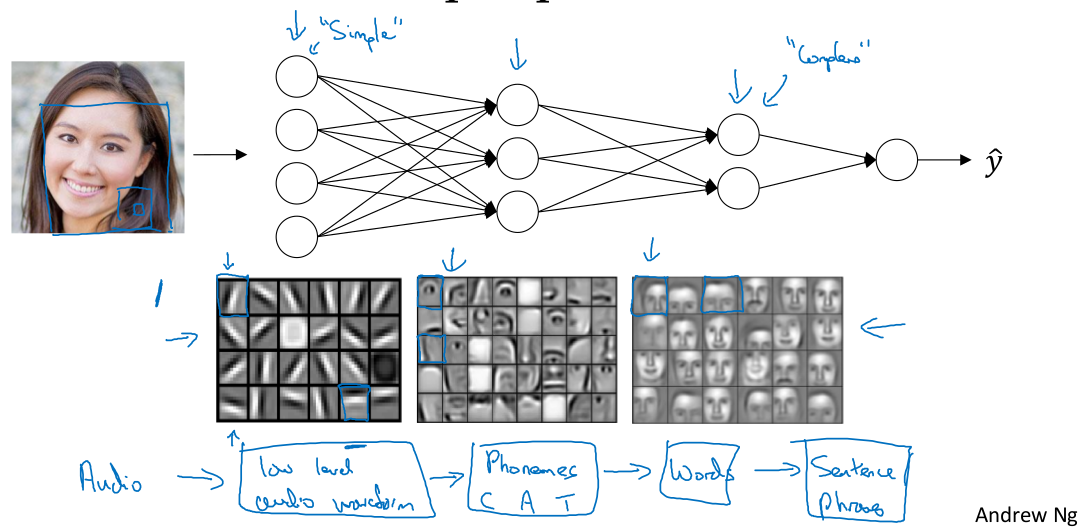
\includegraphics[scale=0.4]{figures/6.png}
	\end{center}
	\caption{Gradient descent diagram.}
	\label{p5}
\end{figure}
It turns out that this cost function J is a convex function which is one of the huge reasons why we use this particular cost function for logistic regression. So to find a good value for the parameters, what we'll do is initialize w and b to some initial value which is usually initialized the value to zero, maybe denoted by that little red dot in Fig.~\ref{p5}. In a word, what gradient descent does is it starts at that initial point and then takes a step in the steepest downhill direction. This is now hidden by the back of the plot until eventually, hopefully converge to this global optimum or get to something close to the global optimum. So this picture illustrates the gradient descent algorithm.

\subsection{Logistic Regression Gradient Descent}

The computations of a neural network are organized in terms of a forward pass or a forward propagation step, in which we compute the output of the neural network, and followed by a backward pass or back propagation step, which we use to compute gradients or compute derivatives. The computation graph explains why it is organized this way.

We're trying to compute a function $J(a,b,c)=3(a+bc)$ and compute this actually has three distinct steps as shown in Fig.~\ref{p6}.
\begin{figure}
	\begin{center}
		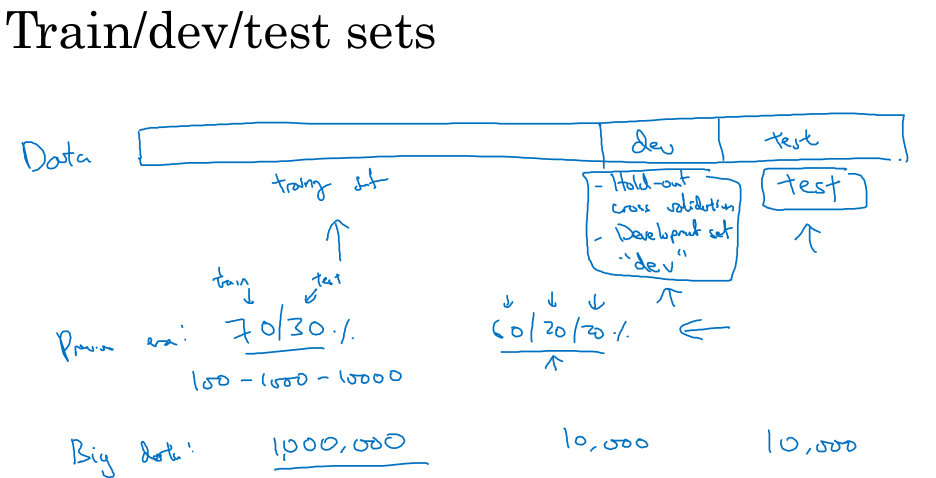
\includegraphics[scale=0.4]{figures/7.png}
	\end{center}
	\caption{Function Computation.}
	\label{p6}
\end{figure}

The computation graph comes in handy when there is some distinguished or some special output variable such as $J$ in this case that we want to optimize. And in the case of a logistic regression, $J$ is of course the cost function that we're trying to minimize.

From Fig.~\ref{p7}, I can know that if we want to know the derivative of J with respect to a, b and c. We can use calculus and the chain rule and get the results such as $\frac{dJ}{da}=\frac{dJ}{dv}\frac{dv}{da}=3\times 1=3$ and $\frac{dJ}{db}=\frac{dJ}{dv}\frac{dv}{du}\frac{du}{dc}=3\times 1\times 2=6$.
\begin{figure}
	\begin{center}
		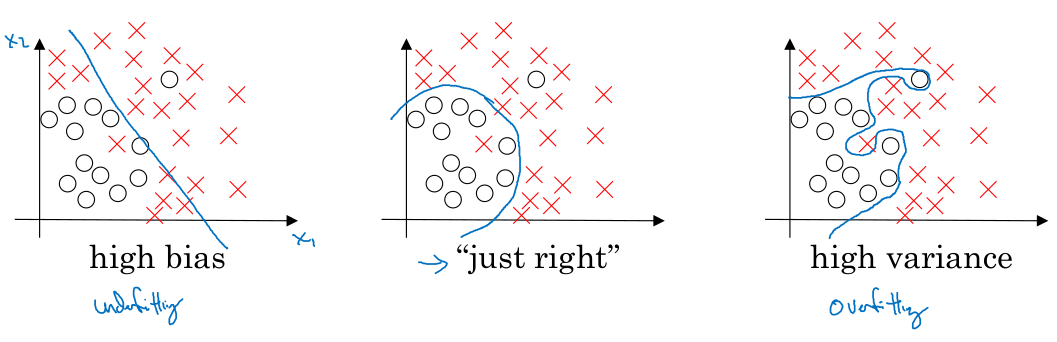
\includegraphics[scale=0.3]{figures/8.png}
	\end{center}
	\caption{Gradient descent diagram.}
	\label{p7}
\end{figure}

Then the key equations we need in order to implement gradient descent for logistic regression by using the computation graph as Fig.~\ref{p8}. In the figure, we should know that $Z=W^\mathrm{T}x+b$, $\hat{y}=a=\sigma(z)$ and loss function $\mathcal{L}=-(y\log(a)+(1-y)\log(1-a))$. With chain rule which is mentioned before, we can get $\frac{d\mathcal{L}}{dz}=\frac{d\mathcal{L}}{da}\times \frac{da}{dz}=a-y$ to go through the calculation. Then, the final step in that computation is to go back to compute how much we need to change w and b in z. Following the mathod above, we can know that  $\frac{d\mathcal{L}}{dw_1}=x_1\times dz$ and so as $dw_2$. This will be one step of grade with respect to a single example that are $w_1:=w_1-\alpha dw_1$, $w_2:=w_2-\alpha dw_2$ and $b:=b-\alpha db$, which is to compute derivatives and implement gradient descent for logistic regression with respect to a single training example.
\begin{figure}
	\begin{center}
		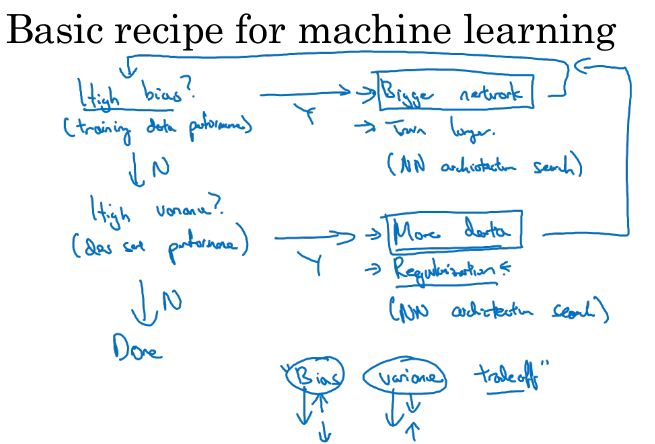
\includegraphics[scale=0.4]{figures/9.png}
	\end{center}
	\caption{Logistic regression derivatives.}
	\label{p8}
\end{figure}

In summary, forward propagation or left to right forward computation for neural network has equations as Eq.~\ref{q2} and then the back propagation step of which as Eq.~\ref{q3}. 
\begin{flalign}
\begin{split}
&Z^{[1]}=W^{[1]}X+b^{[1]},\\
&A^{[1]}=g^{[1]}X(Z^{[1]}),\\
&Z^{[2]}=W^{[1]}A^{[1]}+b^{[2]},\\
&A^{[2]}=g^{[2]}X(Z^{[2]})=\sigma(Z^{[2]}).
\label{q2}
\end{split} 
\end{flalign}

\begin{flalign}
\begin{split}
&dZ^{[2]}=A^{[2]}X-Y,\\
&dW^{[2]}=\frac{1}{m}dZ^{[2]}A^{\mathrm{T}{[1]}},\\
&db^{[2]}=\frac{1}{m}np.sum(dZ^{[2]},axis=1,keepdims=True),\\
&dZ^{[1]}=W^{\mathrm{T}{[2]}} dZ^{[2]}\times g^{\prime[1]} (Z^{[1]}),\\
&dW^{[1]}=\frac{1}{m}dZ^{[1]}X^\mathrm{T},\\
&db^{[1]}=np.sum(dZ^{[1]},axis=1,keepdims=True).\\
\label{q3}
\end{split}
\end{flalign}

Where keepdims prevents python from outputting one of those arrays whose rank is 1. Then by having keepdims=true, this ensures that Python outputs, for a vector that is some n by one like $(n,1)$ other than $(n,)$. All this can see in Fig.~\ref{p16}.
 \begin{figure}
 	\begin{center}
 		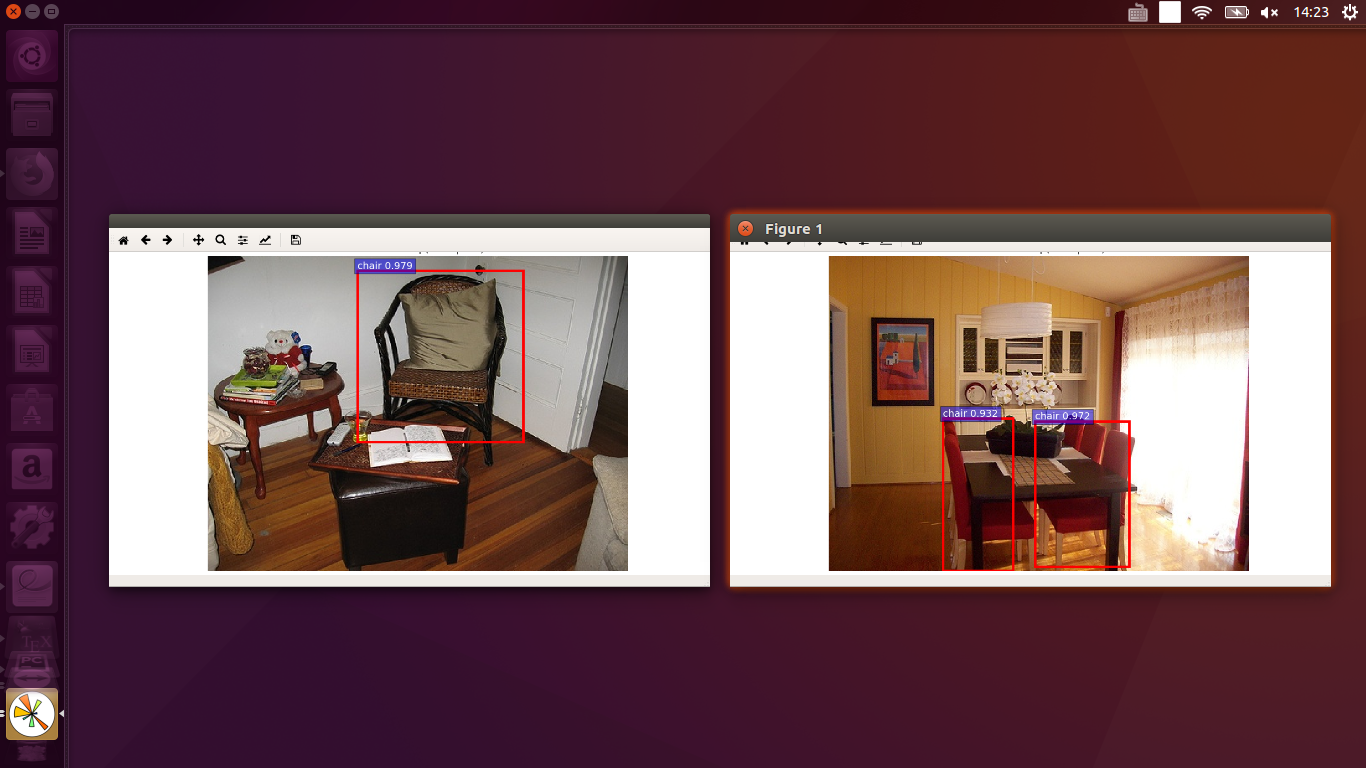
\includegraphics[scale=0.3]{figures/18.png}
 	\end{center}
 	\caption{Formulas for forward and back propagation.}
 	\label{p16}
 \end{figure}

\subsection{Vectorizing Logistic Regression's Gradient Output}
Vectorization is basically the art of getting rid of explicit folders in your code. And in the deep learning era, the ability to perform vectorization has become a key skill. In the same cases, the vectorize version and the non-vectorize version computed the same values. As we can see in Fig.~\ref{p9}, vectorize version takes 2.03ms. While the explicit for loop and non-vectorize version took about 533 milliseconds. The non-vectorize version took something like 262 times longer than the vectorize version.
\begin{figure}
	\begin{center}
		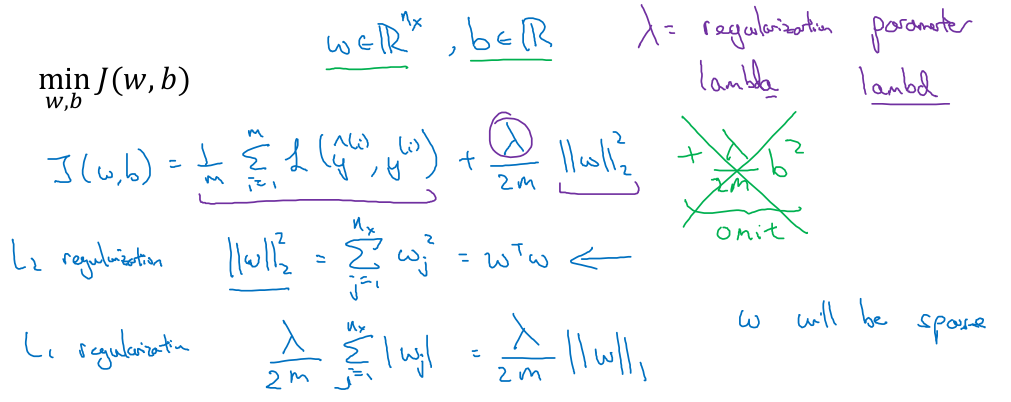
\includegraphics[scale=0.4]{figures/10.png}
	\end{center}
	\caption{Times consuming between the vectorize version and the non-vectorize version.}
	\label{p9}
\end{figure}

Both GPU and CPU have parallelization instructions which are sometimes called SIMD instructions, stands for a single instruction multiple data. If you use built-in functions such as np.function in Fig.~\ref{p9} or other functions that don't require explicitly implementing a for loop. It enables Phyton numpy to take much better advantage of parallelism to do your computations much faster.

In the previous implementation, we've gotten rid of one full loop already but we have this second full loop over 20 examples as left codes in Fig.~\ref{p10}. And we take operations and vectorize them as right codes in the figure. So the vectorized implementation of the derivative calculations is just these right codes in Fig.~\ref{p10}. Now we will see that we can get rid of two for loops to save time when we are doing implementation for logistic regression.
\begin{figure}
	\begin{center}
		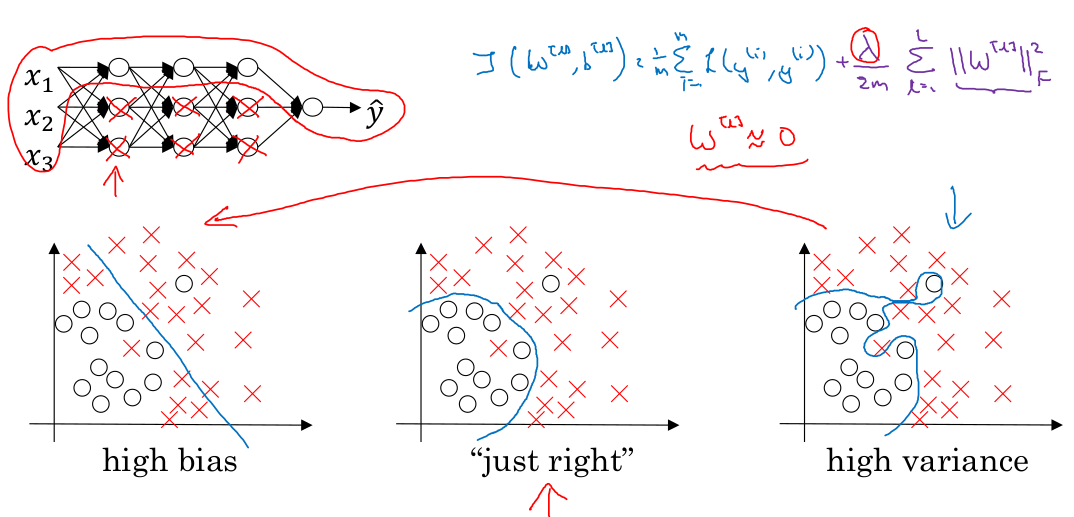
\includegraphics[scale=0.4]{figures/11.png}
	\end{center}
	\caption{Vectorizing logistic regression with and without for loops.}
	\label{p10}
\end{figure}

Now we can know the reason why we should get rid of explicit for loops whenever you can, but if we want to implement multiple adjuration as a gradient descent then maybe still need a for loop over the number of iterations.

\subsection{Neural Networks Representation and Output}

A new network looks as Fig.~\ref{p11} shows. We can form a neural network by stacking together a lot of little sigmoid units whereas previously. We'll use a superscript square bracket 1 to refer to quantities associated with this stack of nodes called a lair and then later use superscript square bracket 2 to refer to quantities associated with Daniel really that's called another layer of the network. The superscript square brackets like we have in the diagram are not to be confused with the superscript round brackets which we used to refer to individual training examples.
\begin{figure}
	\begin{center}
		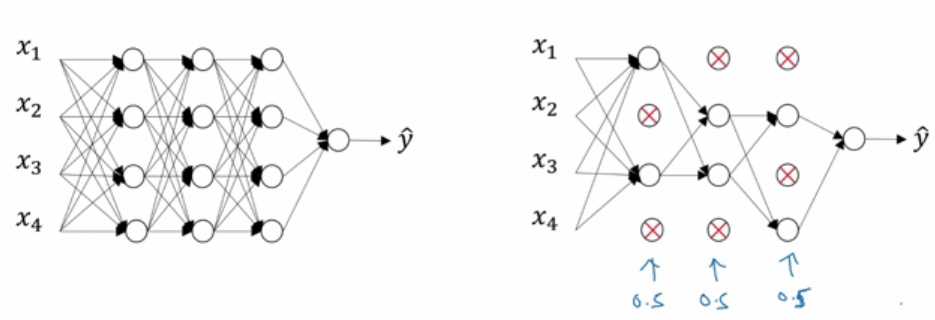
\includegraphics[scale=0.4]{figures/12.png}
	\end{center}
	\caption{Overview of neural network. Superscript square bracket 1 and 2 refers to these different um layers layer 1 and layer 2 in this network}
	\label{p11}
\end{figure}

Here's a picture of a neural network in Fig.~\ref{p12}\subref{p12a}. We have different parts of these pictures some names and input features, $x_1$, $x_2$, $x_3$ stacked up vertically. And this is called the input layer of the neural network. And the middle one is called a hidden layer of the neural network. Besides the final layer here is called the output layer and is responsible for generating the predicted value $\hat{y}$.
 \begin{figure}
 	\centering 
 	\subfigure[Neural Network Representation]{ 
 		\label{p12a} %% label for first subfigure 
 		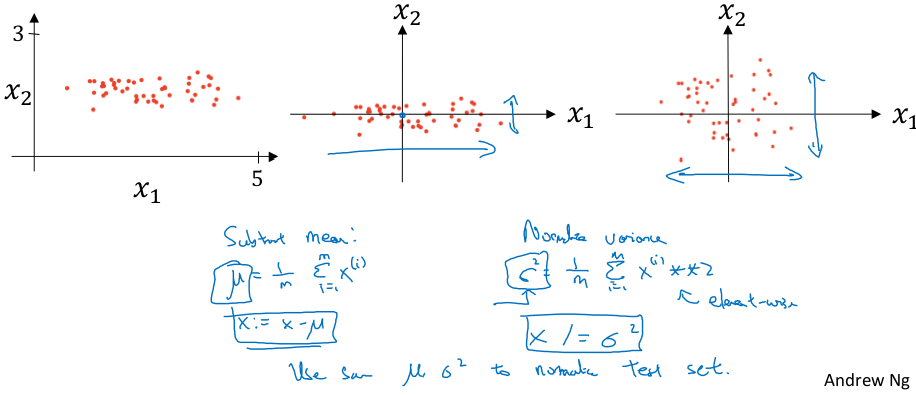
\includegraphics[scale=0.2]{figures/13.png} 
 	} 
 	\subfigure[]{ 
 		\label{p12b} %% label for second subfigure 
 		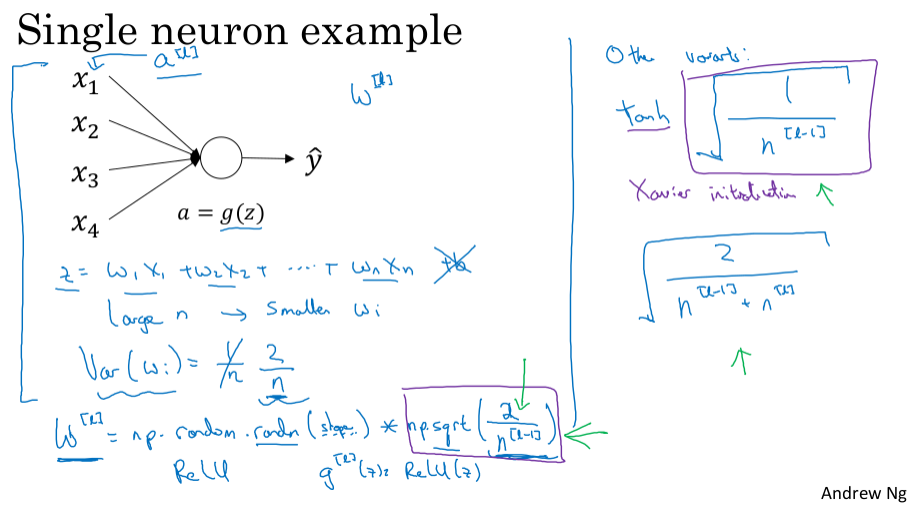
\includegraphics[scale=0.2]{figures/14.png} 
 	} 
 	\caption{Neural Network} 
 	\label{p12} %% label for entire figure 
 \end{figure}
 
 So the input layer passes on the value x to the hidden layer, we're going to call that activations of the input layer $a^{[0]}$. The next layer, the hidden layer will in turn generate some set of activations which we are going to write as $a^{[1]}$. So in particular, the first unit or first, we generate a value $a^{[1]}$. This second we generate a value. Now we're on the $[2]$ and so on. And so,  $a^{[1]}$ has four dimensional vector we want in. And the reason is that when we count layers in neural networks, we don't count the input layer. So the hidden layer is layer one and the output layer is layer two. In our notational convention, we're calling the input layer layer zero, so technically maybe there are three layers in this neural network, because there are the input layer, the hidden layer and the output layer. 
 
Just like logistic regression mentioned above, the circle images the regression really represents two steps of computation first you compute Z as  shwon in Fig.~\ref{p12}\subref{p12a} and in second you compute the activation as a sigmoid function of Z so a neural network just does this a lot more times. 
 
The first node in hidden layer so I've grayed out the other nodes for now so similar to logistic regression on the left this node in a hidden layer which  does two steps of computation right the first step and think it's as the left half of this node it computes $Z^{[1]}_1=W_1^\mathrm{T}x^{[1]}+b_1^{[1]}$ and the notation we'll use is um these are all quantities associated with the first hidden layer so that's why we have a bunch of square brackets there and this is the first node in the hidden layer as shown in Fig.~\ref{p12}\subref{p12b}.

When we have a new network who have one fit in there what you need to implement two computers output is just the four equation and you can think of this as a vectorized implementation of computing the output of first these four logistical russian units. Then hitting there that's what this does and then this which is regression in the output layer as shown in Fig.~\ref{p13}.
 \begin{figure}
 	\begin{center}
 		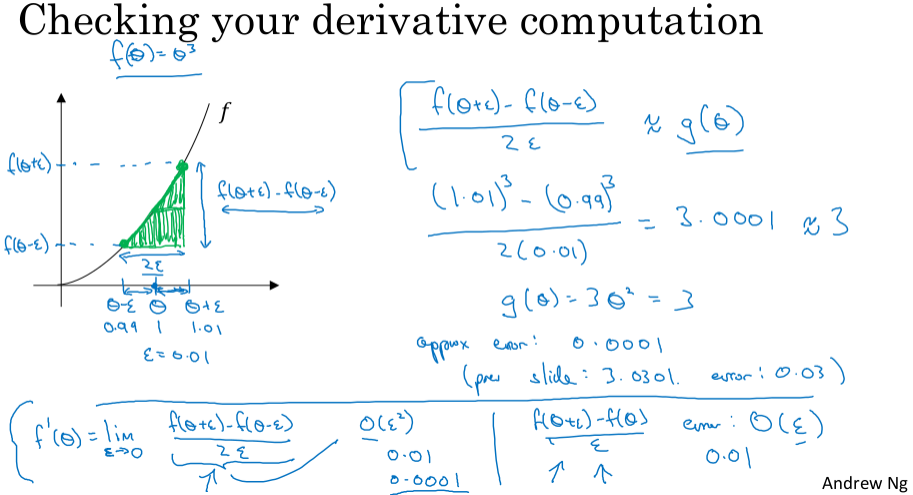
\includegraphics[scale=0.4]{figures/15.png}
 	\end{center}
 	\caption{Neural Network Representation learning.}
 	\label{p13}
 \end{figure}

So just a recap for logistic regression to implement the output or the influence prediction you compute $Z=W^\mathrm{T}x+b$ and $a=\hat{y}$ equals $a=\sigma(z)$ when you have a new network who have one fit in there. What you need to implement two computers output is just the four equation and you can think of this as a vectorized implementation of computing the output of first these four logistical russian units.

\subsection{Activate Function}
It turns out that for your new network to compute interesting functions you do need to take a nonlinear activation function. Fig.~\ref{p14} shows the forprop equations for the neural network, we can know that if $a^{[1]}=z^{[1]}$ and $a^{[2]}=z^{[2]}$, then this model is just computing $\hat{y}$ as a linear function of input features. If we were to use linear activation functions or identity activation functions then the new network is just outputting a linear function of the input $a^{[2]}=w^\prime+b^\prime$. Besides, the one place we might use as linear activation funciton usually in the output layer but other than that using a linear activation function in a hidden layer. All that is the reason why having a nonlinear activation is a critical part of neural networks.
 \begin{figure}
	\begin{center}
		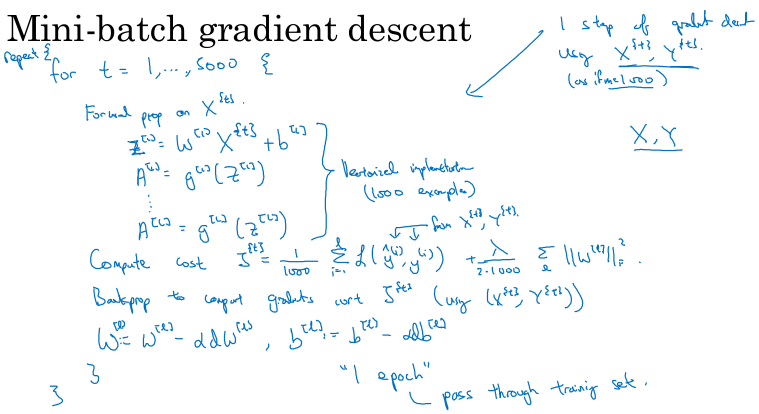
\includegraphics[scale=0.3]{figures/17.png}
	\end{center}
	\caption{Activation funciton.}
	\label{p14}
\end{figure}

When implement back-propagation for neural network, we need ro really compute the slope for the derivative of the activation. There are pros and cons of different activation functions shown in Fig.~\ref{p15} which is never used except for the output layer if we are doing binary classification or maybe almost never use this. Besides, the reason we almost never use this is because the $\tanh$ is pretty much strictly superior so the tanh activation function is $\tanh=\frac{e^z-e^{-z}}{e^z+e^{-z}}$ and then the default the most commonly used activation function is the ReLU which is this so we're not sure what else to use and use this maybe you know feel free also to try to leeky ReLU where function is $max=(0.1z,z)$.
 \begin{figure}
 	\begin{center}
 		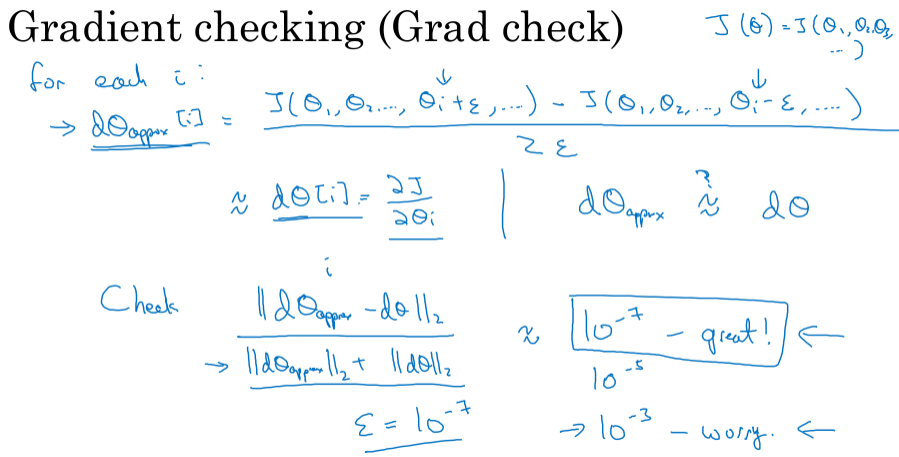
\includegraphics[scale=0.4]{figures/16.png}
 	\end{center}
 	\caption{Neural Network Representation learning.}
 	\label{p15}
 \end{figure}
 
\subsection{Random Initialization}
When we train neural network, it is important to initialize the weights randomly. A neural network of the arrays initialized of parameters to all zero while doesn't work for gradient descent. The problem with this form of initialization is that for any example given, we have that $a^{[1]}_1$ and $a^{[1]}_2$ will be equal and these two activation would be same because both of these hidden units are computing exactly the same function. And then when we compute back propagation, it turns out that $dZ^{[1]}_1$ and $dZ^{[1]}_2$ would also be the same kind of by symmetry right as shown in Fig.~\ref{p17}, which just means that the computing exactly the same function. People usually prefer to initialize the ways to very small random values because if the weights are too large then when you compute the activation values Z will be large or small. So in this case we're more likely to end up at these flat parts of the tanh function or sigmoid function which casues function to be saturated thus slowing down learning.
 \begin{figure}
 	\begin{center}
 		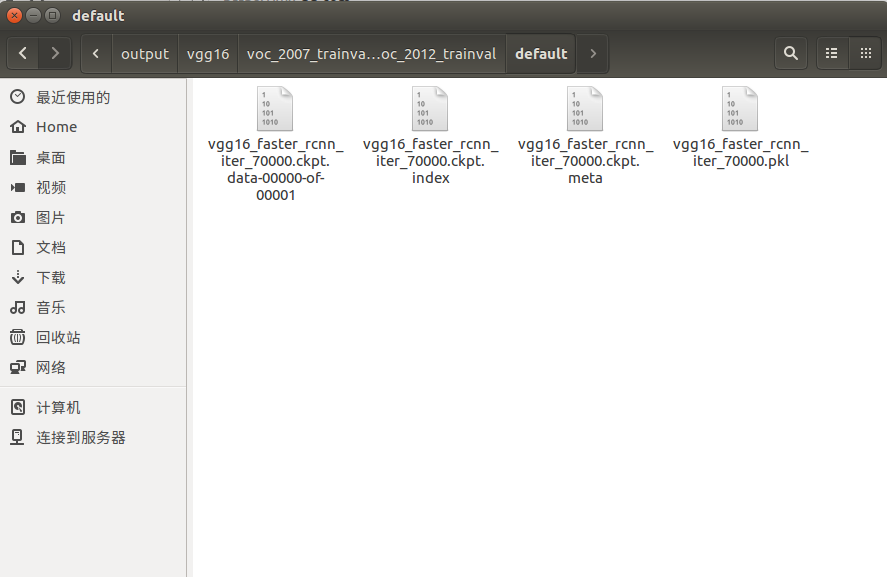
\includegraphics[scale=0.4]{figures/19.png}
 	\end{center}
 	\caption{Initialize weights to zero.}
 	\label{p17}
 \end{figure}


\section{Progress in this week}

This week for deep learning course of Anandrew Ng, I know how to set up a neural network of a hidden layer and initialize the parameters. Besides, I learn to make predicitons using forward propagation as well as compute derivatives and apply gradient descent using back propagation. The details are in following sections. Furthermore, I have succeed in running a Faster R-CNN demo on my laptop with CPU which I take efforts to achieve this as shown in Tab.~\ref{t1}.

\begin{description}
	\item [Step 1] Study the third week course of neural networks and deep learning.
	\item[Step 2] Try my best to run a Faster R-CNN demo.\label{t1}
\end{description}

\section{Plan}

\begin{tabular}{rl}
	\textbf{Objective:} & Finish deep learning course and preparation for URPC2018 \\
	\textbf{Deadline:} & 2018.08.19
\end{tabular}

\begin{description}
	\item[\normalfont 2018.07.16---2018.07.22] Finish neural networks and Deep Learning.
	\item[\normalfont 2018.07.23---2018.07.29] Finish improving deep neural networks courses.
	\item[\normalfont 2018.07.30---2018.08.05] Finish structuring machine learning projects courses.
	\item[\normalfont 2018.08.06---2018.08.12] Finish convolutional neural networks courses.
	\item[\normalfont 2018.08.13---2018.08.19] Finish sequence models courses.
\end{description}



% If you don't cite any references, please comment the following two lines
\bibliographystyle{ieee}
\bibliography{ref.bib}

\end{document}